\section{Architecture}
\label{section:pads}

\eat{\begin{figure}
  \begin{center}
    \scalebox{.5}{\includegraphics{arch1.pdf}}
  \end{center}
  \caption{\pads{} Architecture}
  \label{figure:arch}
\end{figure}}

\begin{figure}
  \begin{center}
    \scalebox{.5}{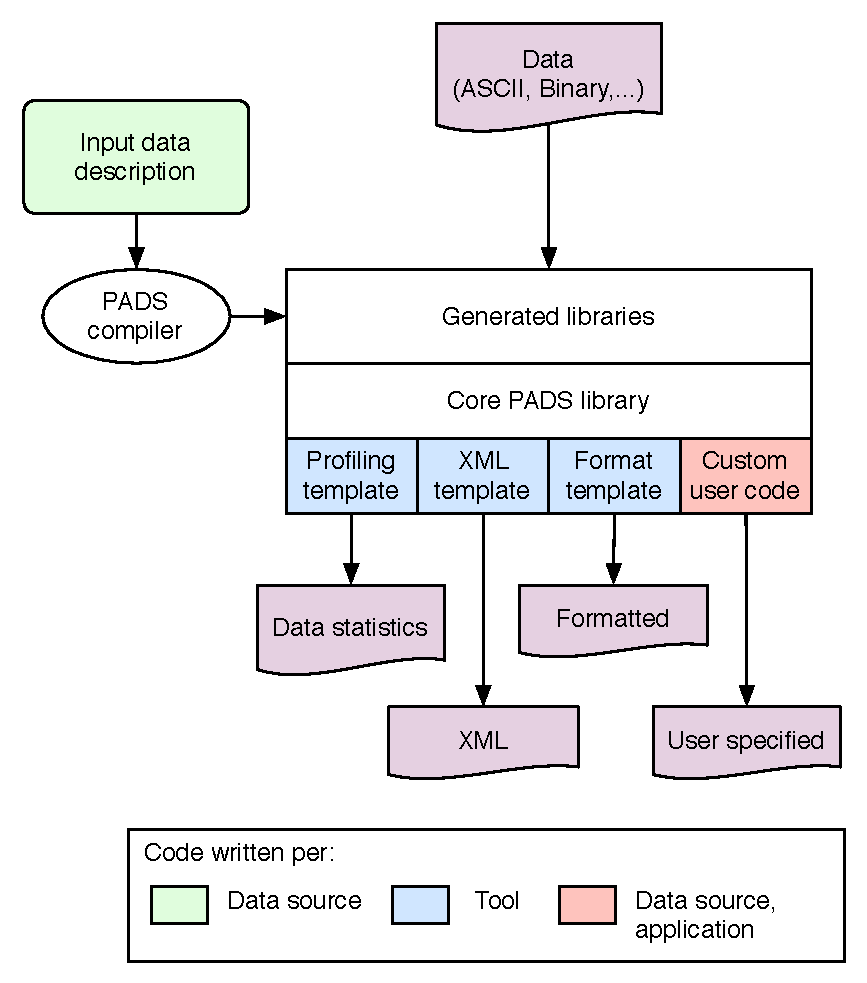
\includegraphics{arch2.pdf}}
  \end{center}
  \caption{\pads{} Architecture}
  \label{figure:arch}
\end{figure}

The \pads{} system, depicted in \figref{figure:arch}, consists of its
description language, compiler, run-time system, and pre-defined tool
suite.  From a description, the compiler generates a library of
description-dependent parsing functions.  The generated library is
linked with a core run-time library and description-independent tool
programs.  Currently, the statistical profiling tool provides
accumulator functions and functions that employ randomized and
approximate techniques to create histogram~\cite{histograms},
wavelet~\cite{histograms-wavelets}, and quantile
summaries\cite{quantiles}.  The XML tool produces a canonical XML view
of a \pads{} source~\cite{fernandez+:padx} and implements the data
model required by the Galax XQuery engine (not shown here).
The format template allows the user to pretty print the data into a  
delimited format suitable for loading in a relational database.   
\eat{The user can supply a sequence of delimiters.  Items at the top level  
in the description are separated by the first delimiter in the  
sequence.  At each nesting level, the tail of the delimiter sequence  
is used.  If the pretty printer reaches a level where the delimiter  
sequence has only one element, that element is used to separate all  
remaining items.}  The format program allows users to override how  
elements of each type are displayed and to omit certain fields  
entirely from the data source.
Lastly, a user may write a custom
application in \C{} to implement their own analyses.

We describe a few key language features to illustrate the language's
expressiveness and completeness.  The language provides a type-based
model: basic types specify atomic data, while structured types
describe compound data built from simpler pieces.
\figref{figure:dibbler} contains the \pads{} description for the
\dibbler{} data format\eat{, which may be generated interactively as
previously described or written by an expert user}.  Types are declared
before they are used, so the type that describes the entire data
source (\cd{summary\_t}) appears last in the description.

The \pads{} library provides a large collection of useful
base types such as 8-bit signed integers, 32-bit unsigned integers, IP
addresses, dates , and strings, \etc{}.  Base types do not specify how
the data is physically coded, \ie{}, in ASCII, EBCDIC, or binary.  \pads{} uses
the \textit{ambient} coding, the default of which is ASCII, but users
can customize it as appropriate.

\begin{figure}
\begin{scriptsize}
\begin{code}
{ 1}. \kw{Precord} \kw{Pstruct} summary\_header\_t \{
{ 2}.  "0|";
{ 3}.  Punixtime tstamp;
{ 4}. \};
{ 5}. \kw{Pstruct} no\_ramp\_t \{
{ 6}.  "no\_ii";
{ 7}.  Puint64 id;
{ 8}. \};
{ 9}. \kw{Punion} dib\_ramp\_t \{
{10}.   Pint64     ramp;
{11}.   no\_ramp\_t  genRamp;
{12}. \};
{13}. \kw{Pstruct} order\_header\_t \{
{14}.        Puint32             order\_num;
{15}.  '|';  Puint32             att\_order\_num;
{16}.  '|';  Puint32             ord\_version;
{17}.  '|';  \kw{Popt} pn\_t           service\_tn;
{18}.  '|';  \kw{Popt} pn\_t           billing\_tn;
{19}.  '|';  \kw{Popt} pn\_t           nlp\_service\_tn;
{20}.  '|';  \kw{Popt} pn\_t           nlp\_billing\_tn;
{21}.  '|';  \kw{Popt} Pzip           zip\_code;
{22}.  '|';  dib\_ramp\_t          ramp;
{23}.  '|';  Pstring(:'|':)      order\_type;
{24}.  '|';  Puint32             order\_details;
{25}.  '|';  Pstring(:'|':)      unused;
{26}.  '|';  Pstring(:'|':)      stream;
{27}. \};
{28}. \kw{Pstruct} event\_t \{
{29}.        Pstring(:'|':)    state;   
{30}.   '|'; Punixtime         tstamp;
{31}. \};
{32}. \kw{Parray} event\_seq\_t \{
{33}.   event\_t[] : \kw{Psep}('|') && \kw{Pterm}(\kw{Peor});
{34}. \};
{35}. \kw{Precord} \kw{Pstruct} order\_t \{
{36}.        order\_header\_t  order\_header;
{37}.   '|'; event\_seq\_t     events;
{38}. \};
{39}. \kw{Parray} orders\_t \{
{40}.   order\_t[];
{41}. \};
{42}. \kw{Psource} \kw{Pstruct} summary\_t\{
{43}.   summary\_header\_t  summary\_header;
{44}.   orders\_t          orders;
{45}. \};
\end{code}
\end{scriptsize}
\caption{\pads{} description for \dibbler{} provisioning data.}
\label{figure:dibbler}
\end{figure}

\eat{A \kw{Penum} type specifies a fixed collection of
literals.}

To describe more complex data, \pads{} provides a collection of
structured types loosely based on \C{}'s type structure.  A
\kw{Pstruct} describes an ordered sequence of data with unrelated
types.  In \figref{figure:dibbler}, the type declaration for the
\kw{Pstruct} \cd{order\_t} (Lines~35--38) contains an order header
followed by the literal character \kw{'|'}, followed by an event
sequence. \pads{} supports character, string, and regular expression
literals.  A \kw{Punion} describes alternatives in the data format
(Lines~9--12), and a \kw{Popt} type specifies optional data
(Lines~17--21).  A \kw{Parray} describes varying-length sequences of
data all with the same type.  The \kw{Parray} type on Lines~32--34
contains the sequence of events an order goes through during
processing.  This declaration indicates that each element in the
sequence has type \cd{event_t}.  It also specifies that the elements
are separated by vertical bars, and that the sequence is terminated by
an end-of-record marker.  \pads{} provides a rich collection of
array-termination conditions: reaching a maximum size, finding a
terminating literal, or satisfying a user-supplied predicate over the
already-parsed portion of the \kw{Parray}.

\pads{} types have two other important features.  A type may have an
associated \emph{predicate} that determines whether a parsed value is
a legal value for the type.  For example, a predicate might require
that one field of a \kw{Pstruct} is greater than another.  Types also
may be \emph{parameterized by values}, which permits the format and
properties of later portions of the data to depend upon earlier
portions.  For example, a type parameter can be used to specify the
(dynamic) size of an array, the appropriate branch of a union, and the
terminating character of a string, \eg{} \cd{Pstring(:'|':)}, among
others.

\eat{Finally, \pads{} \kw{Ptypedef}s allow users to define new types
that add further constraints to existing types.}

\eat{Finally, the \kw{Precord} (Line~35) and \kw{Psource} (Line~42) annotations deserve comment.  The first
indicates that the annotated type constitutes a record,
while the second means that the type constitutes the totality of a data source.  
The notion of a record varies depending upon the data encoding.  
ASCII data typically uses new-line characters to delimit 
records, binary sources tend to have fixed-width records, while 
COBOL sources usually store the length of each record before the actual data.
\pads{} supports each of these encodings of records and allows users to define
their own encodings.  \cut{By default, \pads{} assumes records are new-line terminated.
Before parsing, however, the user can direct \pads{} to use a different record
definition.}}

From a description, the \pads{} compiler generates a \C{} library for
parsing and manipulating the associated data source.  From each type
in a \pads{} description, the compiler generates (1) an in-memory
representation of the type, (2) parsing and printing functions, (3) a
mask, which allows customization of generated functions, and (4) a
parse descriptor, which records the state of the parse, the number of
detected errors, and the code and location of the first error detected
in a value of that type.

Parsing functions take a mask and return an in-memory representation
and a parse descriptor.  The mask allows the user to specify which
constraints the parser should check and which portions of the
in-memory representation it should fill in.  This control allows the
description-writer to specify all known constraints about the data
without worrying about the run-time cost of verifying potentially
expensive constraints for time-critical applications.

Because a distinct parsing function is generated for each type in a
\pads{} description, \pads{} supports multiple-entry point parsing,
which accommodates efficient processing of very large-scale
data~\cite{fisher+:pldi05}.  For a small file, the parsing function
for the \pads{} type that describes the entire file can be called.
For larger-scale data, sequence of calls to parsing functions that
read manageable portions of the file, \eg{}, reading one record at a
time in a loop, is possible.  Currently, the user must specify
explicitly the unit of parsing.

Parse descriptors enable \emph{error-aware} processing of a data
source.  Depending upon the nature of the errors and the desired
application, users can take the appropriate action: halt the program,
discard parts of the data, or repair the errors.  This flexibility
makes it possible to continue processing of very large sources even
when errors are encountered.

The \pads{} system solves important data-management tasks: it supports
declarative description of ad hoc data formats, its descriptions serve
as living documentation, and it permits exploration of ad hoc data and
vetting of erroneous data using a standard query language.  The
resulting \pads{} descriptions and queries are robust to changes that
may occur in the data format, making it possible for more than one
person to profitably use and understand a \pads{} description and
related queries.

\eat{The mapping to \C{} for each is straightforward: \kw{Pstruct}s map to
\C{} structs with appropriately mapped fields, \kw{Punion}s map to
tagged unions coded as \C{} structs with a tag field and an embedded
union, \kw{Parray}s map to a \C{} struct with a length field and a
dynamically allocated sequence, \kw{Penum}s map to \C{} enumerations,
\kw{Popt}s to tagged unions, and \kw{Ptypedef}s to \C{} typedefs.
Masks include auxiliary fields to control behavior at the level of a
structured type, and}

\eat{If the mask requests that a data item be verified
and set, and if the parse descriptor indicates no error, then the
in-memory representation satisfies the semantic constraints on the
data.}

\eat{
\paragraph{Related Work.}
More closely related work includes \erlang{}'s bit syntax~\cite{erlang} and
the \packettypes{}~\cite{sigcomm00} and
\datascript{} languages~\cite{gpce02}, 
all of which allow declarative descriptions of physical data.  These projects were motivated by parsing protocols,
\textsc{TCP/IP} packets, and \java{} jar-files, respectively.  Like
\pads{}, these languages have a type-directed approach to
describing ad hoc data and permit the user to define semantic constraints.
In contrast to \pads{},
these systems handle only binary data and assume the data is
error-free or halt parsing if an error is detected. 
Parsing non-binary data poses additional challenges because of the need
to handle delimiter values and to express richer termination conditions
on sequences of data. These systems also
focus exclusively on the parsing/printing problem, whereas we have 
leveraged the declarative nature of
our data descriptions to build additional useful tools.
}